\documentclass[10pt,a4paper]{article}
\usepackage[utf8]{inputenc}

% Define the page margin
\usepackage[margin=3cm]{geometry}

% Better typography (font rendering)
\usepackage{microtype}

% Math environments and macros
\usepackage{amsmath}
\usepackage{amsfonts}
\usepackage{amssymb}
\usepackage{amsthm}

% Define \includegraphics to include graphics
\usepackage{graphicx}

% Draw graphics from a text description
\usepackage{tikz}

% Syntax highlighting
\usepackage{minted}

% Set global minted options
\setminted{linenos, autogobble, frame=lines, framesep=2mm}

% Import the comment environment for orgtbl-mode
\usepackage{comment}

% Do not indent paragraphs
\usepackage{parskip}

\title{Distributed Systems, Sheet 8}
\author{Marten Lienen (03670270)}

\begin{document}

\maketitle

\section*{Exercise 1}

\subsection*{Part a)}

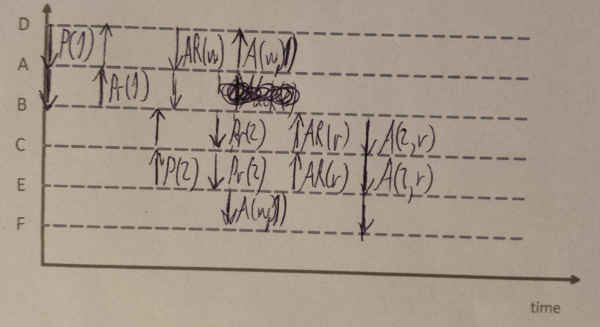
\includegraphics[width=\textwidth]{sheet-8/exercise-1-a}

\subsection*{Part b)}

D proposes, then fails.
E becomes leader and proposes, D comes back up.
D still thinks it is the leaders and proposes again.
E tries to set a value to its proposal but is denied and retries.
D tries to set a value but is denied as well.
This will keep happening until a single leader is selected again.

\section*{Exercise 2}

\subsection*{Part a)}

We use $n$ servers that all keep their own state machine state and participate in the paxos algorithm as proposers, acceptors and learners at the same time.
Whenever the leader receives a client request, it proposes a state transition.
When a transition is learned, each server applies it to its state.

\subsection*{Part b)}

The safety property remains in place because no two proposers can get a quorum at the same time.
However it may not terminate if the proposers continually propose conflicting values and the system becomes unresponsive.

\subsection*{Part c)}

A simple approach would be to restart the server and copy the machine state of a working server.

\section*{Exercise 3}

The safety of paxos always holds for a single non-failing learner because you need at least two learners so that two different values can be learned.
So it has to be the liveness requirement that is broken here, i.e. consensus is never reached.
When at least one of the failing acceptors is part of the quorum, it can always promise in response to proposals and then NACK, when the proposal is set to a value.

\end{document}
